\documentclass{article}

\usepackage{ctex}
\usepackage{tikz}
\usetikzlibrary{cd}
\usetikzlibrary{decorations.pathreplacing}

\usepackage{amsthm}
\usepackage{amsmath}
\usepackage{amssymb}

\usepackage{unicode-math}

\usepackage{enumitem}

\usepackage[textwidth=18cm]{geometry} % 设置页宽=18

\usepackage{blindtext}
\usepackage{bm}
\parindent=0pt
\setlength{\parindent}{2em} 
\usepackage{indentfirst}



\usepackage{xcolor}
\usepackage{titlesec}
\titleformat{\section}[block]{\color{blue}\Large\bfseries\filcenter}{}{1em}{}
\titleformat{\subsection}[hang]{\color{red}\Large\bfseries}{}{0em}{}
%\setcounter{secnumdepth}{1} %section 序号

\newtheorem{theorem}{Theorem}[section]
\newtheorem{lemma}[theorem]{Lemma}
\newtheorem{corollary}[theorem]{Corollary}
\newtheorem{proposition}[theorem]{Proposition}
\newtheorem{example}[theorem]{Example}
\newtheorem{definition}[theorem]{Definition}
\newtheorem{remark}[theorem]{Remark}
\newtheorem{exercise}{Exercise}[section]

\newcommand*{\xfunc}[4]{{#2}\colon{#3}{#1}{#4}}
\newcommand*{\func}[3]{\xfunc{\to}{#1}{#2}{#3}}

\newcommand\Set[2]{\{\,#1\mid#2\,\}} %集合
\newcommand\SET[2]{\Set{#1}{\text{#2}}} %

\begin{document}
\title{Mathematical Analysis}
\author{枫聆}
\maketitle
\tableofcontents

\newpage
\section{实数}
\subsection{实数连续性}

由于在有理数上划分存在一种边界无法确定的情况,即把数轴上所有有理数划分为$A|A'$,其中要求$A$中所有的有理数都小于$A'$中的有理数,在$A$中无最大有理数,且$A'$中无最小有理数,这种情况下{\color{red}无法确定划分两者的边界},例如下组$A$取小于$x^2 < 2$的所有正有理数,上组$A'$取小于$x^2 > 2$的所有正有理数. 

因此引入了无理数的概念,约定上面这种特殊的划分情况定义了某个无理数的$\alpha$,让这个$\alpha$代替缺少的界数,把它插在了$A$里面一切数$a$和$A'$里面一切数$a'$中间。

用上面这种思路来理解某个具体的有理数也是可以的,对任意一有理数$r$存在两种确定它的划分,还是前面的划分方式即$a < r$在下组$A$中,$a > r$在上组$A'$中,而有理数$r$本身可能含于$A$或者$A'$,如果在$A$中,即$A$中有最大有理数,反之在$A'$中,则有最小有理数. 为了确定起见,在提及确定有理数$r$的时候,常把其置于固定的一组,即$A$和$A'$任选一个,以后一直用它,在这里取$r$在上组.

{\color{red} 实数之间的序关系,用划分它集合对应的包含关系来描述},在有理数里面已经有这样的性质了,再看一下无理数,定义划分$A|A'$确定无理数$\alpha$,划分$B|B'$确定无理数$\beta$,即对应下述三种关系

\begin{enumerate}
	\item  $\alpha = \beta$,$A = B$ and $A' = B'$.
	\item  $\alpha > \beta$, $A \supset B$.
	\item  $\alpha < \beta$, $A \subset B$.
\end{enumerate}

还有一个传递关系$\alpha > \beta , \beta > \gamma$,则$\alpha > \gamma$,这些性质都比较容易证明。

\begin{lemma}
对于不论怎样地两个实数$\alpha$和$\beta$,其中$\alpha > \beta$,恒有一个位于它们中间的有理数$r \colon \alpha > r > \beta$.
\end{lemma}

\begin{proof}
这个性质更强了,两个实数($\alpha > \beta$)之间不仅有实数,还有有理数。 来证明一下,定义$\alpha$对应$A|A'$有理数域上的划分,$\beta$对应$B|B'$,因为$\alpha > \beta$,所以有$A$包含$B$,所以可以在$A$上取一点有理数$r$它不含于$B$,于是它属于$B'$,使得$\beta \leq r<\alpha$,$A$里面没有最大数(按照前面的统一),所以把$r$取的大一点就可以把等号去掉.
\end{proof}

开始进攻{\color{red}戴德金基本定理} )

\begin{theorem}
对于实数域内的任一划分$\textbf{A}| \textbf{A}'$必有产生这划分的实数$\beta$存在,$\beta$或是下组$\textbf{A}$中最大数,或是上组$\textbf{A}'$中最小数.	
\end{theorem}

\begin{proof}
首先还是先把实数域上的划分规定先拿出来,定义$\textbf{A}$和$\textbf{A}'$是两个非空集合,每一个实数必落在$\textbf{A}$或者$\textbf{A}'$其中一个里面,且$\textbf{A}$里面的数都小于$\textbf{A}'$里面的数.

将$\textbf{A}$里面的一切有理数记为$A$,$\textbf{A}'$里面的一切有理数记为$A'$,容易证明这样$A|A'$是一个有理数域上划分,划分确定了一个实数$\beta$. 它应该落在$\textbf{A}$或者$\textbf{A}'$中,假设它落在$\textbf{A}$上,则它是$\textbf{A}$中的最大数,假设它不是最大数,则还存在一个$\alpha_0$使得$\alpha_0 > \beta$,根据前面的lemma两个实数之间又可以确定一个有理数$\alpha_0 > r > \beta$,与前提有理数划分的界数矛盾,所以$\beta$是$\textbf{A}$中最大数.
\end{proof}

\newpage
\subsection{数集的界}

\begin{theorem}
若数集$\mathcal{X}=\{x\}$上(下)有界,则它必有上(下)确界.
\end{theorem}

\begin{proof}
我们分两种情况来看待这个问题.
如果$\mathcal{X}$存在一个最大数$\bar{x}$,对一切$x \in \mathcal{X}$都有$x \leq \bar{x}$. 这个时候$\bar{x}$是$\mathcal{X}$是一个上界同时也是上确界.

如果$\mathcal{X}$中不存在这样的最大数,那么我们取$\mathcal{X}$的所有上界$\alpha'$构成归入上组$\textbf{A}'$. 一切其他的实数归入下组$\textbf{A}$. 我们知道$\mathcal{X}$是都会落在下组$\textbf{A}$中的,因为对于任意的$x \in \mathcal{X}$,在当前前提下它都不可能是一个上界. 所以现在$\textbf{A}$和$\textbf{A}'$都是非空的. 那么现在实际上弄了实数上的一个划分出来,根据戴德金定理我们知道这样划分会产生一个界数$\beta$,无论这个界数落在$\mathcal{A}$或者$\mathcal{B}$里面也好,都可以用它作为这个独特的上确界,因为一切上界都大于等于它. 
\end{proof}

这里有一个小推论,clearly.

\begin{corollary}
若数集$\mathcal{X}$有一个上界$M$,则$\sup{x} \leq M$.
\end{corollary}


\newpage
\section{极限论}
\subsection{数列极限}
数列,整序傻傻分不清....

\begin{definition}
若对于每一整数$\varepsilon$,不论它怎样小,恒有序号$N$,使在$n > N$时,一切$x_n$的指满足不等式\[|x_n-a| < \varepsilon\],则称常数$a$为整序变量$x=x_n$的极限.

$a$是整序变量的极限这一事实,记成:\[\lim x_n =a \text{ 或者 } \lim x = a\],也可以说这个序列收敛于$a$
\end{definition}

有一个很有趣的几何解释在这里,

\begin{center}
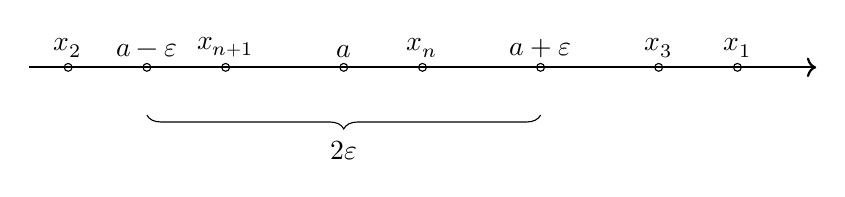
\begin{tikzpicture}
\draw[thick,->] (0,0) -- (10,0);
\draw (0.5,0) node[circle,draw,scale=0.3]{} node[above] {$x_2$};
\draw [decorate,decoration={brace,amplitude=5pt,mirror,raise=4ex}]
  (1.5,0) node[circle,draw,scale=0.3]{} node[above]{$a-\varepsilon$} -- (6.5,0) node[midway,yshift=-3em]{$2 \varepsilon$} node[circle,draw,scale=0.3]{} node[above]{$a+\varepsilon$};
%\draw [Parenthesis-Parenthesis,] (2,0) node[above] {$a-\varepsilon$} -- (7,0) node[above] {$a+\varepsilon$};
\draw (2.5,0) node[circle,draw,scale=0.3]{} node[above] {$x_{n+1}$};
\draw (4,0) node[circle,draw,scale=0.3]{} node[above] {$a$};
\draw (5,0) node[circle,draw,scale=0.3]{} node[above] {$x_n$};
%\draw (7,0) node[circle,draw,scale=0.3]{} node[above] {$a+\varepsilon$};
\draw (8,0) node[circle,draw,scale=0.3]{} node[above] {$x_3$};
\draw (9,0) node[circle,draw,scale=0.3]{} node[above] {$x_1$};
\end{tikzpicture}
\end{center}

以$a$点为中心的线段不论取的多小(其长度为$2\varepsilon$),一切$x_n$点从某点起,必全部落在这线段之内,这样在线段之外一定只有有限长度个点了,表示极限的点$a$表示整序变量的数值的点的凝聚中心.

\newpage
\subsection{无穷小量}

\begin{definition}
极限为零的整序变量$x_n$称为无穷小量,或简称无穷小.
\end{definition}

这里有一个有趣的命题.

\begin{proposition}
无限个无穷小之积不一定是无穷小.
\end{proposition}

它是一个自然语言的命题,所以里面有一些争议. 先看一个一般性构造证明.

\begin{proof}
取一系列数列: \\

$$
\begin{matrix} 
\{a_1\}:&1,&\frac12, & \frac13, &\frac14, & \frac15, & \frac16, &\cdots\\ \{a_2\}:&1,&2,&\frac13, &\frac14, &\frac15, &\frac16, &\cdots\\ \{a_3\}:&1,&1,&3^2, &\frac14, &\frac15, &\frac16, &\cdots\\ \{a_4\}:&1,&1,&1,&4^3,&\frac15, &\frac16, &\cdots\\ \vdots
\end{matrix}
$$

数列$\{a_k\}$的第$n$项记为$a_k(n)$,其通项公式为
$$
a_k(n)=\begin{cases} 1,&n<k\\ k^{k-1},&n=k\\ \frac1n,&n>k\\ \end{cases}
$$

显然对于任意的$k \in \mathbb{Z}^+$都满足$\lim\limits_{n\to\infty}a_k(n)=0$. 所以这一系列数列都是无穷小. 那么这一系列数列乘积的第$n$项为

\begin{align*}
\prod_{k=1}^\infty a_k(n) &=\left(\prod_{k=1}^{n-1}a_k(n)\right) a_n(n)\left(\prod_{k=n+1}^\infty a_k(n)\right) \\
&=\left(\frac1n\right)^{n-1}\cdot n^{n-1}\cdot1^\infty=1.
\end{align*}

因此$\lim_{n\to\infty}\prod_{k=1}^\infty a_k(n)=1$.
\end{proof}

但是有一个奇怪现象是什么呢?$\prod_{k=1}^na_k(n)$中有一项$a_n(n)=n^{n-1}$是一个无穷大,并不是无穷小. 奇怪的东西乱入了.

再看一个经典的无穷个无穷小之和:

$$
\lim_{n\to\infty}\left(\frac1{n^2}+\frac2{n^2}+\frac3{n^2}+\cdots+\frac n{n^2}\right)=\lim_{n\to\infty}\sum_{k=1}^n\frac k{n^2} = \lim_{n\to\infty}\frac{1+2+3+\cdots+n}{n^2}=\lim_{n\to\infty}\frac{\frac12n(n+1)}{n^2}=\frac12.
$$

定义$b_k(n)=\frac k{n^2}$,则$b_n(n)=\frac n{n^2}$还是无穷小. 两个东西对比一下,你可能需要重新定义命题.

%https://zhuanlan.zhihu.com/p/88642140
%https://wenku.baidu.com/view/32a5ded87f1922791688e8c5.html
%https://wenku.baidu.com/view/376d928a866fb84ae45c8db0.html?from=search

\newpage
\subsection{区间套}

\begin{lemma}
给定单调增数列$x_n$和单调减数列$y_n$,且恒有\[x_n < y_n,\]若其差$y_n - x_n$趋向于$0$,则它们有公共有限极限:\[c = \lim x_n  = \lim y_n.\]
\end{lemma}

常用形式是取一个闭区间$[a,b]$,然后在取一个区间$[a',b']$使得\[a \leq a' < b' \leq b\],则$[a',b']$是套在$[a,b]$里面的.

设有一区间套的无穷序列\[[a_1,b_1],[a_2,b_2],\cdots,[a_n,b_n],\cdots\]后一个总是套在前面一个内,并且在$n$增大时这些区间的长度趋向于$0$:\[\lim b_n - a_n = 0.\]则区间的两端点$a_n$和$b_n$趋于共同极限\[c = \lim a_n = \lim b_n.\]


\newpage
\subsection{收敛原理}

\begin{theorem}
数列变量$x_n$有有限极限的充分必要条件是: 对于每一个数$\varepsilon > 0$,存在序号$N$,使得$n > N$及$n' > N$,不等式\[|x_n - x_{n'}| < \varepsilon\]成立.
\end{theorem}

记录一下用分割法证明其必要性.
\begin{proof}
设前提条件都已经满足,在全体实数域下构造一个划分. 对于任何实数$\alpha$,若$x_n$从某项其满足不等式\[x_n > \alpha,\]则取这种实数$\alpha$归入下组$A$,其余的(即不落在$A$里面的)一起实数归入上组$A'$.

首先我们来说明这样确实产生了一个实数上的划分. 由前提条件,对于任意数$\varepsilon>0$及其对应的$N$. 若$n > N$及$n' > N$,则下面不等式成立\[x_{n'} - \varepsilon < x_n < x_{n'}+\varepsilon\].现在我们可以看到每一个数$x_{n'} - \varepsilon$都是小于$x_n$的,所以它归入下组$A$. 另一方面$x_{n'}+\varepsilon$都大于$x_n$,所以$x_{n'}+\varepsilon$放不进去$A$,那它只能归入$A'$了,所以$A$和$A'$都是非空的. 我们的划分方式对于每一个数$\alpha$和确定序列$x_n$,要么它属于$A$或者属于$A'$. 同时$A$中实数都小于$A'$的实数. 如果$\alpha > \alpha', \alpha \in A , \alpha' \in A'$,则$x_n$从某一项其也都大于$a'$,这样就产生矛盾了. 所以确实产生了一个实数上的划分.

根据戴德金基本定理,有实数$a$存在它是这两组数之间的界数,即\[\alpha \leq a \leq \alpha'.\]我们注意到当$n > N$时,$x_{n'} - \varepsilon$是一个$\alpha$,而$x_{n'} +\varepsilon$是一个$\alpha'$. 所以我们有\[x_{n'} - \varepsilon \leq a < \leq x_{n'} + \varepsilon\].即$|x_{n'}-a| \leq \varepsilon$,所以$\lim x_n = a$.
\end{proof}

\begin{theorem}
B.Bolzano-C.Weierstrass. 任何有界数列内恒能选出收敛于有限极限的部分极限.(有界序列一定有收敛子列)
\end{theorem}

\begin{proof}
假设一切$x_n$都位于界限$a$与$b$之间. 现在将$[a,b]$分为两半,则必有一半含有无限多个数列$x_n$里面的元素. 因为不是这样则数列$x_n$就有有限多个了. 用$[a_1,b_1]$表示其中含有无限多个数列元素的那半个区间(若两个区间都含有无限多个数列元素,任取一个即可).类似的取在区间$[a_1,a_2]$分出它的一半$[a_2,b_2]$,使得它也含有无限多个$x_n$. 继续这种取法至无穷,在第$k$次分出的区间$[a_k,b_k]$内同样也有无穷多个$x_n$. 此外,第$k$个区间的长度为\[\frac{b-a}{2^k}.\]可以看到这个长度趋于$0$的,然后把区间套用在这里,就可以知道$a_k$和$b_k$是趋于某个公共极限$c$.

也就是说从上面我们分出来的区间里面,都挑一个元素出来,构成的子列是取趋于某个极限的.
\end{proof}

利用BC定理,我们可以尝试把前面对收敛原理的证明可以写的更简单.

\begin{proof}
假设前提条件满足,即对任意的$\varepsilon > 0$,当$n > N,n'>N$时$|x_n-x_{n'}|< \varepsilon$.也就是\[ x_{n'} -\varepsilon < x_n < x_{n'} + \varepsilon.\]可以看到$x_n$是有界的,可以想象把这个界限拉长把前$N$个$x_n$也包含进来.

假设从$\{x_n\}$里面挑出来某个子列$\{x_{n_k}\}$收敛于$c$,即\[|x_{n_k} -c| < \varepsilon.\]当$n_k > N,n > N$时,我们有\[|x_n - x_{n_k}| < \varepsilon.\]两式联立有\[|x_n - c| < 2\varepsilon.\]所以$x_n$也是收敛于$c$的.
\end{proof}



\newpage
\section{一元函数}
\subsection{单调函数的极限}

\begin{definition}
\rm 单调函数分为广义的单调函数和严格的单调函数. 例如当$x > x'$有$f(x) \geq f(x')$就是广义单调增函数,也叫不减函数(菲砖). 与之对应的严格单调增函数就需要把前面这个不等式的等号去掉.
\end{definition}


\begin{theorem}
\rm 设$f(x)$在区域$\mathcal{X}$内单调增加,即使是广义的也可以. 区域$X$以大于一切$x$的数$a$(它可以是有限的,也可以是$-\infty$)作为聚点. 若在这时$f(x)$上有界:
$$
	f(x) \leq M , \forall x \in \mathcal{X}.
$$
则当$x \rightarrow a$时函数有一有限的极限. 在与此相反的场合,它趋向于$+\infty$.
\end{theorem}

\begin{proof}
$f(x)$有上界必有上确界$A$. 给定任意的$\varepsilon > 0$所以必存在一点$x'<a$使得$f(x') > A-\varepsilon$. 另一方面我们永远都有$f(x) \leq A < A+\varepsilon.$ 故对满足上述条件的$x$有下面的不等式存在
$$
	|f(x)-A| < \varepsilon 
$$
由于$f(x)$单调增函数,所以当$x >x'$时有$f(x)>f(x')$,即$f(x) > f(x') > A-\varepsilon$. 这就是极限的定义$\lim\limits_{x \rightarrow a} = A$.

反过来你可以取$a$小于一切$x \in \mathcal{X}$. $f(x)$下有界,类似的下确界$A'$也可以得到类似的不等式$|f(x)-A'| < \varepsilon$.
\end{proof}

\newpage
\subsection{连续函数的性质}
\begin{lemma}
\rm E.Borel. 若闭区间$[a,b]$被一个开区间的无穷系$\sum = \{\sigma\}$所覆盖,则恒能从$\sum$里面选出有限子系\[\sum^{*} = {\sigma_1,\sigma_2,\cdots,\sigma_n},\]它同样可以覆盖全区间$[a,b]$.
\end{lemma}

\begin{proof}
\rm H.lebesgue' s. 定义$x^*$为区间$[a,b]$中使得区间$[a,x^*]$能用有限个区间$\sigma$来覆盖的点. $x^*$肯定是存在,因为$a$就是,只要找一个包含$a$的开区间$\sigma$就行,这样想的话,又可以找到一群,$\sigma$中接近$a$的都是这样的点.

所以我们的任务是证明$b$也是这样的一个$x^*$.
因为一切$x^* \leq b$,故亦有\[\sup\{x^*\}=c \leq b.\],因为$c$也是$[a,b]$中一点,同样可以找到包含它的开区间$\sigma_0=(\alpha,\beta)$.但依据上确界的性质,我们还可以找到$x^*$使得$\alpha < x^* \leq c$.所以现在把$\sigma_0$来在加到有限个区间$\sigma$里面去,现在就可以覆盖区间$[a,c]$,也就是说上确界$c$也是$x^*$.

而且$c$是不能小于$b$的,如果$c$小于$b$,如果是这样$c$和$\beta$也可以找到一点$x^*$,这与$c$是上确界矛盾的.这样,必须有$c=b$,即$b$也是属于$x^*$.所以$[a,b]$可以被有限覆盖.
\end{proof}

%https://blogs.scientificamerican.com/roots-of-unity/what-does-compactness-really-mean

为什么$(a,b)$不是紧致的呢? 考虑$(a+\frac{b-a}{n},b)$,任何一个$(a,b)$的真子集都可以被它覆盖,但是它不能有限覆盖$(a,b)$,因为如果有限就意味着我们能找到一个最大的开区间属于$(a,b)$,实际上这样的开区间并不存在. 但是如果我们加上$a$和$b$,这种方式已经无法覆盖$a$和$b$两点了.

Compact means small. It is a peculiar kind of small, but at its heart, compactness is a precise way of being small in the mathematical world. The smallness is peculiar because, as in the example of the open and closed intervals $(0,1)$ and $[0,1]$, a set can be made “smaller” (that is, compact) by adding points to it, and it can be made “larger” (non-compact) by taking points away.

\newpage
\subsection{函数连续性和间断}

函数$f(x)$在点$x_0$处右连续或者左连续
\begin{align}
f(x_0+0) = \lim\limits_{x \rightarrow x+0} f(x) = f(x_0) \\
f(x_0-0) = \lim\limits_{x \rightarrow x-0} f(x) = f(x_0).
\end{align}
函数$f(x)$在点$x_0$有右间断或者左间断是指对应的上式不成立. 例如第一个式子不成立则是右间断.

函数连续的充要条件可以变成{\color{blue} 函数在点$x_0$处连续就是等于说它在这一点是同时左连续和右连续的}.

如果$f(x)$在$x_0$处有有限极限$f(x_0+0)$和$f(x_0-0)$存在,但是它们均不等于$f(x_0)$,则称$x_0$是这里是一个普通间断点或者第一类间断点(跃度). 若极限$f(x_0+0)$或者$f(x_0-0)$是无穷或者根本不存在,则称$x_0$这里是第二类间断点.

\begin{example}
$f(x)$定义在区间$[0,1]$上: 若$x$是无理数则$f(x)=0$; 若$x$是有理数表示为不可约通分数$\frac{p}{q}$则$f(\frac{p}{q})=\frac{1}{p}$. 可以得到一个有趣的结论: $f(x)$在任一有理数有普通间断点,任一无理数上连续.

\rm 事实上无论$x$取任意数$x_0$,对于任意的$\varepsilon > 0$,要使得$f(x) < \varepsilon$,只需要取$p > \frac{1}{\varepsilon}$. 不满足这样的正整数$p$只有有限多个. 我们找一个$x_0$的邻域$(x_0-\delta,x_0+\delta)$把这些点排除在外,那么所有在这个邻域里面的点(排除$x_0$)都可以满足$|f(x)| < \varepsilon$. 即意味着
$$
f(x_0 + 0) = f(x_0 - 0) = 0.
$$
若$x_0$是一个有理数,则$x_0$是一个普通间断点. 反之若$x_0$是一个有理数则在$x_0$处连续.
\end{example}

\newpage
\subsection{单调函数的连续性和间断}

\begin{theorem}
\rm 单调增(减)函数$f(x)$在$\mathcal{X}$内若有间断,只能是第一种间断,即跃度.
\end{theorem}

\begin{proof}
取$\mathcal{X}$上任意一点$x_0$,并设它不是$\mathcal{X}$的左端点. 则当$x < x_0$时有$f(x) \leq f(x_0)$,此时$f(x)$是有界的,根据我们前面证明的单调函数的极限定理,$f(x)$在$x_0$这里是有左极限存在$\lim\limits_{x \rightarrow x_0-0} \leq f(x_0)$(上确界小于任意的上界).

设$x$也不是右端点,那么右极限当$x > x_0$, 有$f(x) \geq f(x_0)$. 也有极限$\lim\limits_{x \rightarrow x_0 + 0} \geq f(x_0)$. 如果左右极限都等于$f(x_0)$则$f(x)$在这点连续.
\end{proof}


\begin{theorem}
\rm 若单调函数$f(x)$在区间$\mathcal{X}$上对应的函数值充满整个区间$\mathcal{Y}$(任意$y \in \mathcal{Y}$都至少有一个$f(x_0)$与之对应),则$f(x)$在$\mathcal{X}$上连续.
\end{theorem}

\begin{proof}
假设$f(x)$在$\mathbf{X}$上存在一间断点$x_0$,我们知道这样的间断点只能是第一间断点. 即在$x_0$这一点两边都有极限但是不等于$f(x_0)$. 在这种情况下我们需要找到一点$y_0 \in \mathcal{Y}$它并不能被$f(x)$覆盖从而推出矛盾. 当$x < x_0$时有$f(x)< f(x_0)$. 这里我们就找出了这样$y$属于$f(x) < y < f(x_0)$.
\end{proof}

这个定理非常的有用,它可以很简单直接来描述一些单调初等函数的连续性,而不需要用定义来刻画.

\newpage
\subsection{连续函数的复合}

\newpage
\subsection{一个有趣的方程的解}

\begin{example}
求定义在区间$(-\infty,+\infty)$上满足
$$
f(x+y) = f(x) + f(y)
$$
的一切连续函数$f(x)$.
\end{example}

\begin{proof}
这个函数只能是$f(x)=cx$.
\end{proof}

\newpage
\subsection{函数连续性在计算极限时的应用}

有三个比较重要的极限.

\begin{enumerate}
	\item $\lim\limits_{\alpha \rightarrow 0} \frac{\log_a(1+\alpha)}{\alpha} = \log_a e$

直接用对数函数的性质,把$\alpha$放到对数函数里面就行,对数函数里面的极限是$e$.当$a=e$时极限的结果就是很漂亮的$1$.			
	
	\item $\lim\limits_{\alpha \rightarrow 0} \frac{a^\alpha-1}{\alpha} = \ln a$
	
遇到这样略微有些复杂的表达式,直接考虑换元. 让$\beta = a^\alpha -1$,则$\beta \rightarrow 0$. 原式就变成了$\lim\limits_{\beta \rightarrow 0} \frac{\beta}{\log_a(\beta+1)}$. 变成了上面我们熟悉样子.	
	
	\item $\lim\limits_{\alpha \rightarrow 0} \frac{(1+\alpha)^\mu-1}{\alpha} = \mu$
	
还是考虑换元,但是不要换的太彻底,适可而止即可. $\beta = (1+\alpha)^\mu - 1$,其中$\beta \rightarrow 0$. 我们可以得到一个有趣的等式$\mu \ln(1+\alpha) = \ln(1+\beta)$. 到这里就够了,不用把$\beta$把$\alpha$表示出来. 我们把原式现在整理如下\[\frac{(1+\alpha)^\mu-1}{\alpha} = \frac{\beta}{\alpha} = \frac{\beta}{\ln(1+\beta)}\cdot\frac{\ln(1+\alpha)}{\alpha}.\]又变成了我们熟悉的样子,两边的极限都是$1$,所以最后的整体的极限为$\mu$.	
\end{enumerate}

\newpage
\subsection{连续函数的性质}

零点定理或者Bolzano-Cauchy第一定理.
\begin{theorem}
函数$f(x)$在闭区间$[a,b]$上连续,且$f(a) \cdot f(b) < 0$即两端函数值异号. 则存在一点$c$使得$f(c)=0$.
\end{theorem}

\begin{proof}
在这里可以用上区间套,取$c =\frac{a+b}{2}$,如果$f(c)$正好等于$c$那就太好了,我们一下子就找到了它. 如果$f(c)$并不等于$0$,那么$[a,\frac{a+b}{2}]$和$[\frac{a+b}{2},b]$必有一个区间两端异号,我们再取这个区间的中间值. by induction, 我们只需要研究最差的情况有$\lim\limits_{n \rightarrow \infty}(b_n - a_n)=0$,则存在极限$\lim a_n = \lim b_n = c$. 再根据我们的取法还有$f(a_n) < 0$和$f(b_n) > 0$. 因为$f(x)$在$[a,b]$上连续,所以$f(x)$在$c$点是有极限存在的,并且左右极限是相等的,那么只能$\lim f(c) = 0$.
\end{proof} 

上面定理其实还有一种证法,但是需要给出一个小lemma. 也就是连续保号的性质.

\begin{lemma}
若函数$f(x)$在$x=x_0$处连续,且$f(x_0)$不等于$0$,则对于充分接近$x_0$的一切$x$的函数值$f(x)$仍保持着在$f(x_0)$的函数值.
\end{lemma}

\begin{proof}
根据连续的定义,任意的$\varepsilon > 0$, 存在$|x-x_0| < \delta$使得$|f(x)-f(x_0)| < \varepsilon$成立. 若$f(x_0)>0$,我们把这个不等式左边的绝对值拿到我们有$f(x) > f(x_0) - \varepsilon$,只要我们让这个$\varepsilon$取的足够小,就能使得$f(x_0) - \varepsilon > 0$. 即$\varepsilon < f(x_0)$就行. 反之若$f(x_0) < 0$,有$f(x) < f(x_0) + \varepsilon$,同样只要这个$\varepsilon$取的足够小,可以使得$f(x_0) + \varepsilon < 0$. 即$\varepsilon < -f(x_0)$.
\end{proof}

利用这个lemma再给出一种证明,这个证明也是我中意的.

\begin{proof}
\rm 现在我们从任意一个端点出发,例如我选点$a$. 先假设没有这样的点$c$存在使得$f(c)=0$. 并设$f(a) < 0$,我们可以选一个特殊的区间出来$[a,d]$, 有上面这个lemma我们可以让这个区间里面所有的$x$都有$f(x)<0$,那么这个$d$最大可以取到哪里呢?肯定存在一个最大值,因为$f(b)>0$,所以一定有$d < b$. 我们现在考虑在这种情况下,充分接近$d$右边的$x$一定都有$f(x) > 0$,如果不是这样我们可以取更大的$d$. 那么在$d$点这里,有$\lim\limits_{x \rightarrow d-0} < 0$和$\lim\limits_{x \rightarrow d+0} > 0$,这表示在这$d$这一点并不连续,与假设矛盾.

上面是我们子集的论证过程,其实有点模糊,再记录一下更正规的论证方式. 还是设$f(a)<0$,我们可以取出所有$f(\bar{x}) < 0$这样的$x$. 因为$f(b) > 0$,所以$\{\bar{x}\}$上有界,我们取$c = \sup\{\bar{x}\}$. 我们来探讨一下$f(c)$的大小,若是$f(c) < 0$,根据前面的lemma在充分接近$c$的右边也存在$x$使得$f(x)<0$,这就和$c$是上确界矛盾了. 同样$f(c) >0$,我们也可以在$c$的左边找到$f(x)>0$,这也和$c$是上确界矛盾.
\end{proof}


\newpage
\section{导数及微分}

导数常用的表示法.

\begin{enumerate}
	\item $\frac{dy}{dx}$或$\frac{df(x_0)}{dx}$ 莱布尼茨(G.W.Leibniz);
	\item $y'$或者$f'(x_0)$ 拉格朗日(J.L.Lagrange);
	\item $Dy$或者$Df(x_0)$ 柯西(A.L.Cauchy).
\end{enumerate}

\subsection{常用导数求法和表示}

\begin{enumerate}
	\item 常函数的导数等于{ \color{blue} $0$}. 这个就非常trivial了.
	\item $y=x^n$,其中$n$是自然数. {\color{blue} $y' = nx^{n-1}.$}

$y+\Delta y = (x+\Delta x)^n$这个式子二项式展开即可. 即$x^n + nx^{n-1}\Delta x + \frac{n(n-1)}{1 \cdot 2}x^{n-1}+ \cdots$.	
	
	\item $y=\frac{1}{x}$. {\color{blue} $y'=-\frac{1}{x^2}$}. 直接用导数的基本定义就行.
	\item $y=\sqrt{x}$. {\color{blue} $y' = \frac{1}{2}x^{-\frac{1}{2}}$.} 直接用导数的基本定义就行.
	\item $y=x^\mu$,其中$\mu$是任意实数. {\color{blue} $y' = \mu x^{\mu - 1}$.}
	
$\frac{\Delta y}{\Delta x} =  \frac{(x+\Delta x)^{\mu} - x^\mu}{\Delta x} =  x^{u-1} \cdot  \frac{(x+\frac{\Delta x}{x})^\mu - 1}{\frac{\Delta x}{x}}$. 其中左边极限是我们前面写过的一个重要极限值为$\mu$.	
	\item $y=a^x$,其中$a >0$. { \color{blue} $y' = a^x \cdot \ln a$.}
	
$\frac{\Delta y}{\Delta x} =\frac{a^{x + \Delta x} - a^x}{\Delta x} =  a^x \cdot \frac{a^{\Delta x} - 1}{\Delta x}$. 最后等式做边又是我们熟悉的极限.
\end{enumerate}

\newpage
\subsection{函数的增量公式}

设$y=f(x)$. 在$x$的定义域上固定一个$x_0$,用$\Delta x \lessgtr 0$表示$x$的任意增量. 于是对应的函数的增量为\[\Delta y = \Delta f(x_0) = f(x_0 + \Delta x) - f(x_0).\]

若$y=f(x)$在$x_0$处有有限的导数$y_x'=f'(x_0)$. 则函数的增量可以表示如下的形式.\[\Delta f(x_0) = f'(x_0) \cdot \Delta x + \alpha \cdot \Delta x.\]或者更简短地\[\Delta y = y_x' \cdot \Delta x + \alpha \cdot \Delta x.\]式中的$\alpha$是依赖$\Delta x$的变量,且随着$\Delta x$一同趋于零.

这个$\alpha$是怎么来的呢?在导数的定义中,$\Delta x \rightarrow 0$时,有\[\frac{\Delta y}{\Delta x} \rightarrow y_x'.\]故令\[\alpha = \frac{\Delta y}{\Delta x} - y_x'.\]这里可以看出来$\alpha \rightarrow 0$. 通过这个等式把$\Delta y$表示出来就是前面的等式. 

因为$\alpha \cdot \Delta x$是比$\Delta$更高阶的无穷小.故上面的等式还可以改成写\[ \color{blue} \Delta y = y_x' \cdot \Delta x + o(\Delta x).\]这个式子相对来说就非常简洁了.
\newpage
\subsection{复合函数的导数}

设函数$ \mu = \varphi(x)$在某一点$x_0$处有导数$u_x' = \varphi'(x_0)$. 函数$y=f(\mu)$在对应的$\mu_0 = \varphi(x_0)$也有导数$y_u'=f'(u_0)$. 于是复合函数$y = f(\varphi(x))$在$x_0$处亦有导数\[[f(\varphi(x_0))]' =  f_u'(\varphi(x_0))\cdot\varphi'(x_0).\]或者\[\frac{dy}{dx} = \frac{dy}{du}\cdot\frac{du}{dx}.\]

\begin{proof}
先根据导数的定义来求$\Delta y $. 给$x$以任意增量$\Delta x$,$\Delta u$是函数$u = \varphi(x)$对应增量, 最后$\Delta y$是由增量$\Delta u$所引起的函数$y = f(u)$的增量. 根据函数增量公式我们有\[\Delta y = y_u' \cdot \Delta u + \alpha \cdot \Delta u.\]然后两边都除以$\Delta x$ \[\frac{\Delta y}{\Delta x} = y_u' \cdot \frac{\Delta u}{\Delta x} + \alpha \cdot \frac{\Delta u}{\Delta x}. \]当$\Delta x \rightarrow 0$时,$\frac{\Delta u}{\Delta x}$就是$u_x'$,而$\alpha \cdot \frac{\Delta u}{\Delta x}$是一个趋于$0$高阶无穷小. 所以最后\[\lim\limits_{\Delta \rightarrow 0} \frac{\Delta y}{\Delta x} = y_u' \cdot \lim\limits_{\Delta \rightarrow 0} \frac{\Delta u}{\Delta x} = y_u' \cdot u_x'. \]
\end{proof}


这个式子也是我们常说的链式法则(记得在以前在看mit的微积分的时候,那个代课老师在讲链式法则的时候,突然拿了一条真的链子出来. 说这个法则的强大在于让我们挣脱了链子的束缚...),可以推广到任意有限个函数复合的情形. 我们可以尝试来推一下二阶链式法则.
\begin{equation}
\begin{aligned}
\left(\frac{dy}{dx}\right)' &= \left( \frac{dy}{du} \right)' \cdot \frac{du}{dx} + \frac{dy}{du} \cdot \left( \frac{du}{dx} \right)' \\
&= \frac{d^2y}{du^2} \cdot \frac{du}{dx} \cdot \frac{du}{dx} + \frac{dy}{du} \cdot \frac{d^2u}{dx^2} \\
&= \frac{d^2y}{du^2} \cdot \left( \frac{du}{dx} \right) ^2 + \frac{dy}{du} \cdot \frac{d^2u}{dx^2}
\end{aligned}
\end{equation}


%\left(\frac{dy}{dx}\right)' = \left( \frac{dy}{du} \right)' \cdot \frac{du}{dx} + \frac{dy}{du} \cdot \left( \frac{du}{dx} \right)' 
%= \frac{dy}{dx}
\newpage
\subsection{高阶导数及高阶微分}

二阶微分记为:\[d^2 y =d(dy).\]二阶微分的微分记为:\[d^3 y = d(d^2 y).\]一般地说,函数$y=f(x)$的$(n-1)$阶微分的微分称为函数$y=f(x)$的$n$阶微分\[d^n y  = d(d^{n-1} y).\]

在求高阶微分时很重要的一件事,{\color{red} 是要记住$dx$是不依赖于$x$的任意的数,关于$x$而微分时必须把它看成常数因子}.在这种情形,将有

\begin{align*}
	d^2 y = d(dy) = d(y' \cdot dx) = dy' \cdot dx = (y'' \cdot dx) \cdot dx = y'' \cdot dx^2, \\
	d^3 y = d(d^2 y) = d(y'' \cdot dx^2) =dy'' \cdot dx^2 = (y'''\cdot dx)\cdot dx^2 = y''' \cdot dx^3.
\end{align*}

很容易可以猜出普遍规律是\[d^n y = y^{(n)} \cdot dx^n.\]由它可以进一步推得\[y^{(n)} = \frac{d^n y}{d x^n}.\]

{\color{blue} 但是高阶微分没有形式不变性},即若$x = \varphi(t)$,于是$y$可以看成$t$的复合函数$y = f(\varphi(t))$. 它关于$t$的一阶微分可以写成\[dy =y_x' \cdot dx,\]其中$dx = x_t' \cdot dt$. 再求它关于$t$的二阶微分\[d^2 y = d(y_x' \cdot dx) = dy_x' \cdot dx + y_x' \cdot d(dx) = y'' \cdot dx + y_x' \cdot d^2 x.\]这才是二阶微分的一般形式. 之前的高阶微分形式$x$是自变量,所以$d^2 x = 0$.
\end{document}
